\documentclass[12pt]{article}
\usepackage{amsmath}
\usepackage{amssymb}
\usepackage{geometry}
\usepackage{enumerate}
\usepackage{natbib}
\usepackage{float}%稳定图片位置
\usepackage{graphicx}%画图
\usepackage[english]{babel}
\usepackage{a4wide}
\usepackage{indentfirst}%缩进
\usepackage{enumerate}%加序号
\usepackage{multirow}%合并行
\title{\large UM-SJTU JOINT INSTITUTE\\PHYSICS LABORATORY\\(VP141)\\\ \\\ \\\ \\\ \\\ \\\ \\\ \\\ \\\ \\\ \\\
LABORATORY REPORT\\\ \\\ EXERCISE 5\\\  DAMPED AND DRIVEN OSCILLATIONS \\\ \\\ \\\ \\\ \\\ }
\author{Name: Pan Chongdan\\ID: 516370910121\\Partner: Yang Ruiming\\ID:516370910127\\Group: 16}
\date{Date: \today}

\begin{document}
\maketitle
\newpage
\section{Objectives}
In this exercise, I will study damped and driven oscillations in mechanical systems using the Pohl resonator. I'll also observe and quantify the mechanical resonance phenomenon.
\section{Theoretical Background}
If a periodically varying external force is applied to a damped harmonic oscillator, the resulting motion is called forced (or driven) oscillations, and the external force is called the driving force. Assuming that the driving force is of the form
$$F=F_0(sin\omega t+\delta)$$
with the amplitude $F_0$ and angular frequency $\omega$, the resulting steady-state forced oscillations will be simple harmonic with the angular frequency equal to that of the driving force. The amplitude of these steady-state oscillations turns out to depend on the angular frequency of the the driving force, in particular on how far it is from the natural angular frequency, and the damping coefficient. The amplitude may become quite large, and this phenomenon is known as the mechanical resonance.
\par Another interesting property of driven steady-state oscillations is the fact that there is a phase lag between the driving force and the displacement from the equilibrium position of the oscillating particle. This phase lag reaches $\pi/2$ (a quarter of the cycle) when the system is driven at the natural angular frequency.
\par In this experiment, forced oscillation of a balance wheel will be studied. Damping in this system is provided by air drag and electromagnets inducing eddy currents in the wheel. It is a rotating system, hence the corresponding quantities (such as the force and the position) will be replaced by their angular counterparts.
\par When the balance wheel is acted upon a periodic driving torque $\tau_{dr}=\tau_0 cos\omega t$ and a damping torque $\tau_f=-b\frac{d\theta}{dt}$, in addition to the restoring torque $\tau=-k\theta$, its equation of motion is of the form
\begin{equation}
I\frac{d^2\theta}{dt^2}=k\theta-b\frac{d\theta}{dt}+\tau_0 cos\omega t
\end{equation}
where $I$ is the moment of inertia of the balance wheel, $\tau_0$ is the amplitude of the driving torque, and $\omega$ is angular frequency of the driving torque. Introducing the symbols
$$\omega_0^2=\frac{k}{I},2\beta=\frac{b}{I},\mu=\frac{\tau_0}{I}$$
equation (1) can be rewritten as
\begin{equation}
\frac{d^2\theta}{dt^2}+2\beta\frac{d\theta}{dt}+\omega_0^2\theta=\mu cos\omega t
\end{equation}
which, in the absence of the driving torque ($\mu=0$), is the equation of motion for a
damped harmonic oscillator. If, additionally, there is no damping in the system ($\beta=0$), equation (2) describes a simple harmonic oscillator with the natural angular frequency $\omega_0$. The solution to equation(2), in the general case of a damped and driven system, is of the form
\begin{equation}
\theta(t)=\theta_{tr}(t)=\theta_{st}cos(\omega t +\varphi)
\end{equation}
where the former term $\theta_{dr}$ denotes the transient solution, that depends on the the initial conditions and vanishes exponentially as $t\to\infty$. The latter term describes steady-state oscillations, with the amplitude
\begin{equation}
\theta_{st}=\frac{\mu}{\sqrt{(\omega_0^2-\omega^2)^2+4\beta^2\omega^2}}
\end{equation}
The phase shift $\varphi$ gives information about to what extent the displacement from the equilibrium position lags behind the the driving force. It can be found as
$$tan\varphi=\frac{2\beta\omega}{\omega^2-\omega_0^2}$$
where $-\pi\leqslant\varphi<0$. Note again that, the amplitude and the phase shift are determined by $\mu$,$\omega$,$\omega_0$, and $\omega$, and but not the initial conditions.
\par By finding the maximum of $\theta_{st}$, as a function of $\omega$, we can find the \emph{resonance angular
frequency} $\omega=\omega{res}=\sqrt{\omega_0^2-2\beta^2}$, and the corresponding amplitude
$$\theta_{res}=\theta_{st}(\omega_{res})=\frac{\mu}{2\beta\sqrt{\omega_0^2-\beta^2}}$$
For small values of the damping coefficient $\beta$, the resonance angular frequency is close to the the natural angular frequency, and the amplitude of steady-state oscillations becomes large. The dependence of both the amplitude and the phase shift on the driving angular frequency are shown in the left and right Figure 1, respectively, for different values of the damping coefficient. Please note that with increasing damping, (1) the resonance frequency moves away from the natural frequency towards smaller values, (2) the amplitude of the steady-state oscillations decreases.
\section{Apparatus}
The BG-2 Pohl resonator consists of two main parts: a vibrometer and a control box.
The vibrometer is shown in Figure 2. A copper balance wheel is mounted on a supporting
\begin{figure}[H]
\centering
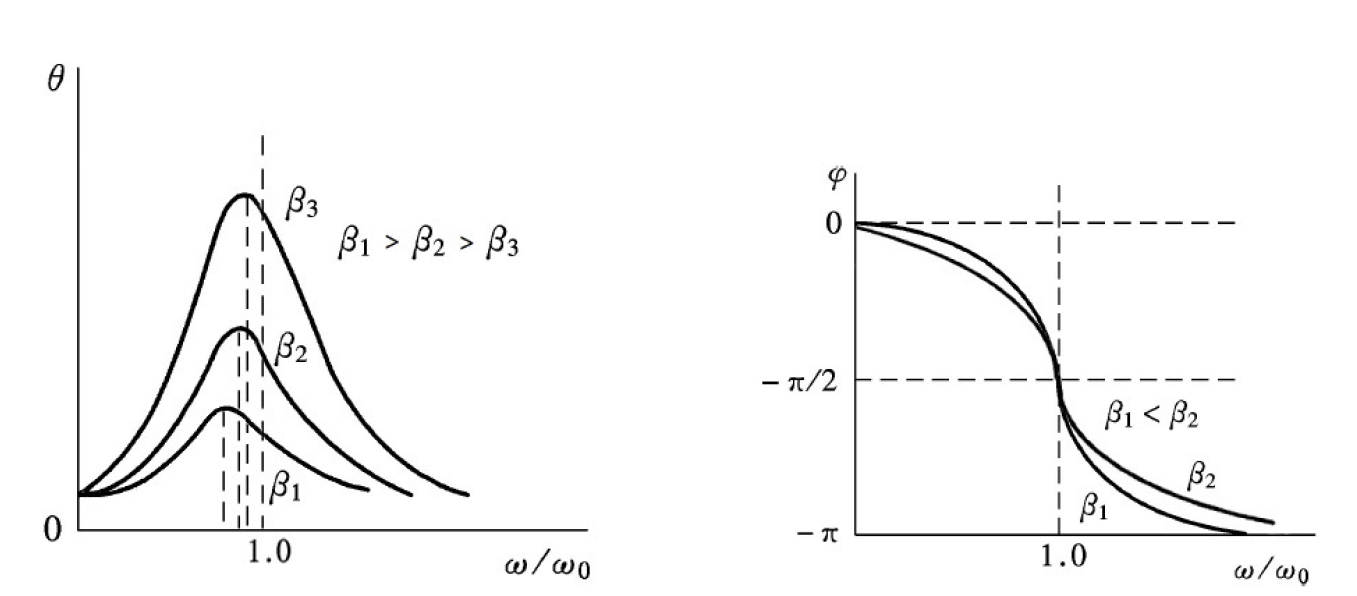
\includegraphics[scale=0.4]{P1.jpg}
\caption{The dependence of the amplitude (left) and phase shift (right) of steady-state driven oscillations.}
\end{figure}
frame, and the axis of the balance wheel is attached to the supporting frame with a scroll spring. The spring provides an elastic restoring torque to the wheel, which makes the balance wheel rotating about an equilibrium position.
\par There are many notches on the edge of the balance wheel with one notch being much
deeper than the others. A photoelectric detector is set above the deep notch. The detector is used to measure the amplitude and the period of oscillations, and it is connected to the electronic control box.
\par A pair of coils is placed at the bottom of the supporting frame, with the balance wheel fitting exactly into the gap between the two coils. Due to electromagnetic induction, the wheel will be acted upon an electromagnetic damping force when the coils are carrying current, and the magnitude of the damping force can be controlled by changing the current.
\par The device is equipped with a motor with an eccentric wheel and a rod used to drive the wheel.
\begin{figure}[H]
\centering
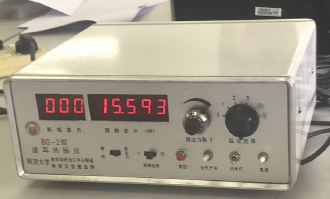
\includegraphics[scale=1]{P7.jpg}
\caption{The dependence of the amplitude (left) and phase shift (right) of steady-state driven oscillations.}
\end{figure}
\par There is a \textbf{Period Selection} switch and a \textbf{Period of Driving Force} knob on the electric control box, which allow to control the speed of the motor precisely. Another photoelectric detector is set above the turntable and connected to the control box to measure the period of driving force.
\par The phase shift can be measured using the glass turntable with an angle scale and
a strobe light. The strobe is controlled by the photoelectric detector above the wheel. When the deep notch passes the equilibrium position, the detector sends a signal and the strobe ashes. In a steady state, a line on the angle scale will be highlighted by the ash of the strobe and the phase difference can be read from the angle scale directly.
\par The amplitude of oscillations is measured by counting the notches on the wheel, and this measurement is performed by a photoelectric detector with the result displayed on the electronic control box.
\begin{figure}[H]
\centering
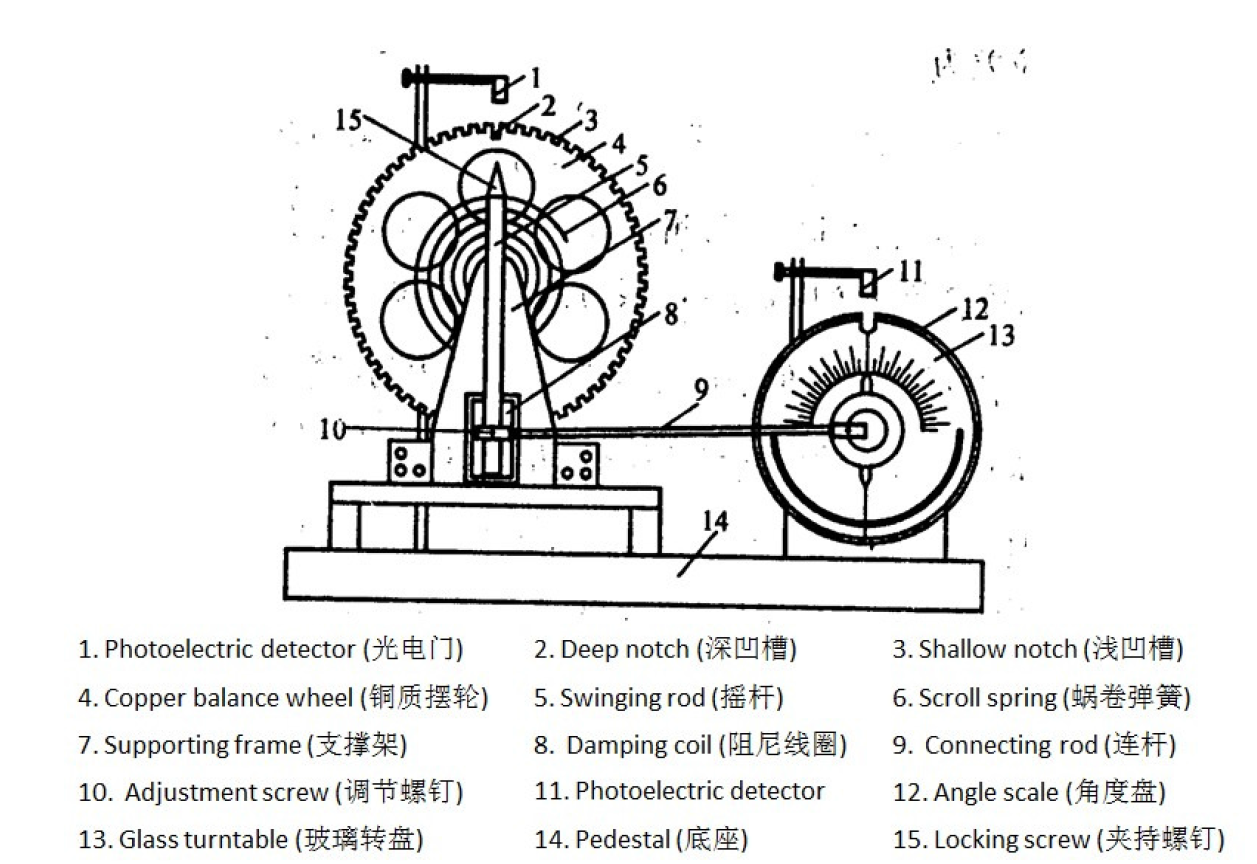
\includegraphics[scale=0.5]{P2.jpg}
\caption{The vibrometer.}
\end{figure}
\par The front panel and the rear panel of the control box are shown in Figures 3 and 4, respectively.
\par The function \textbf{Amplitude Display} shows the oscillation amplitude of the balance wheel and Period Display shows the oscillation period in two modes. When the \textbf{Period Selection} switch is at position "1", a single oscillation period will be displayed; when the \textbf{Period Selection} switch is at "10", the time of 10 oscillation periods will be displayed. The reset button works only when the \textbf{Period Selection} button is at "10".
\par The period of the driving force can be changed precisely by using the \textbf{Period of the driving force} knob, but please pay attention that the scale on the knob is not very accurate.
\par The \textbf{Damping Selection} knob changes the damping force by adjusting the electric current through the coils at the bottom of the wheel. There are six options, ranging from "0" (no current) to "5" (current of about 0.6 A). You will use "2", "3" or "4" in this exercise.
\par The strobe generates a ash that allows you to read the phase difference from the
angle scale directly. To protect the strobe, you should turn on the \textbf{Strobe} switch only when measuring the phase difference. 
\par The \textbf{Motor Switch} is used to control the motor. You should turn the motor off when measuring the damping coefficient and the natural angular frequency.
\begin{figure}[H]
\centering
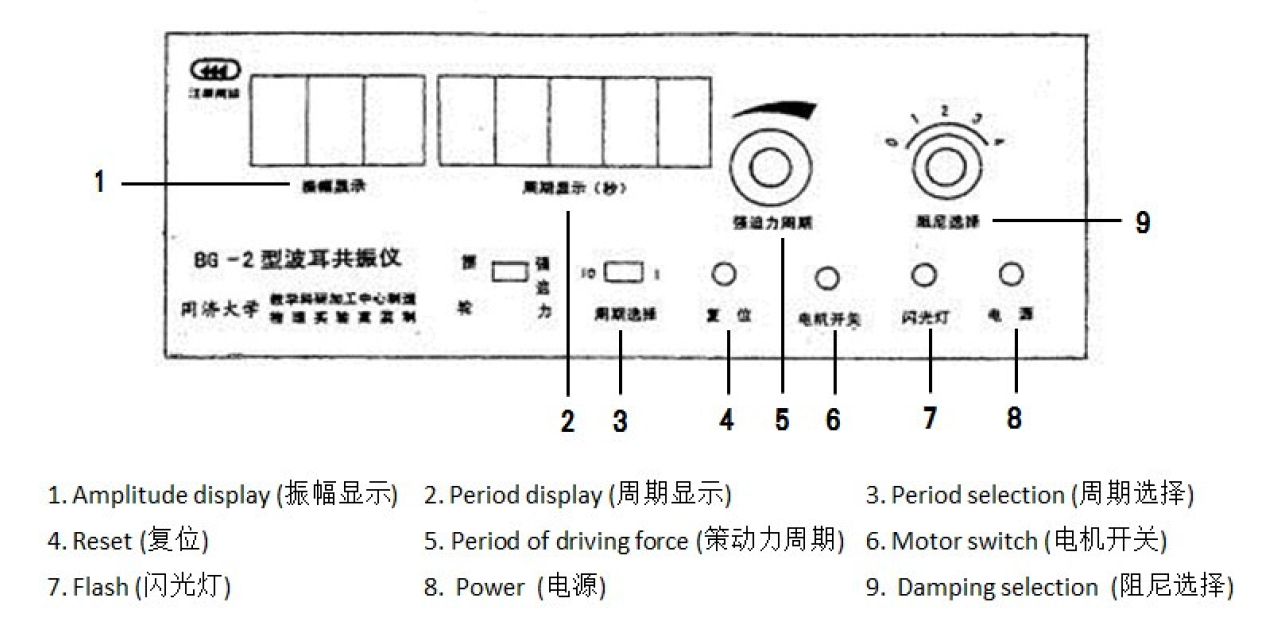
\includegraphics[scale=0.5]{P3.jpg}
\caption{The front panel of the control box.}
\end{figure}
\section{Measurement Procedure}
\subsection{Natural Angular Frequency}
\begin{enumerate}
\item Turn the \textbf{Damping Selection} knob to "0".
\item Carefully rotate the balance wheel to the initial angular position $\theta_0\approx 150^o$ and
release it. Record the time of 10 periods.
\item Repeat for four times and calculate the natural angular frequency $\omega_0$.
\end{enumerate}
\subsection{Damping Coefficient}
\begin{enumerate}
\item Turn the \textbf{Damping Selection} knob to "2", and the selection should not be changed during this part.
\item Carefully rotate the balance wheel to the initial amplitude of approximately $150^o$ and release it. Record the amplitude of each period (start from the second amplitude after you release the wheel) and the time of 10 periods.
\item The solution to the homogeneous equation of motion (2), with the corresponding initial conditions, is $\theta(t)=\theta_0e^{-\beta t}cos(\omega_ft+\alpha)$. Hence $\theta_1=\theta_0e^{-\beta T},\theta_2=\theta_0e^{-\beta(2T)},\cdots\theta_n=\theta_0e^{-\beta(nT)}$. The damping coefficient $\beta$ can then be calculated as 
$$ln\frac{\theta_i}{\theta_j}=ln\frac{\theta_0e^{-\beta(iT)}}{\theta_0e^{-\beta(jT)}}=(j-i)\beta T$$
\begin{figure}[H]
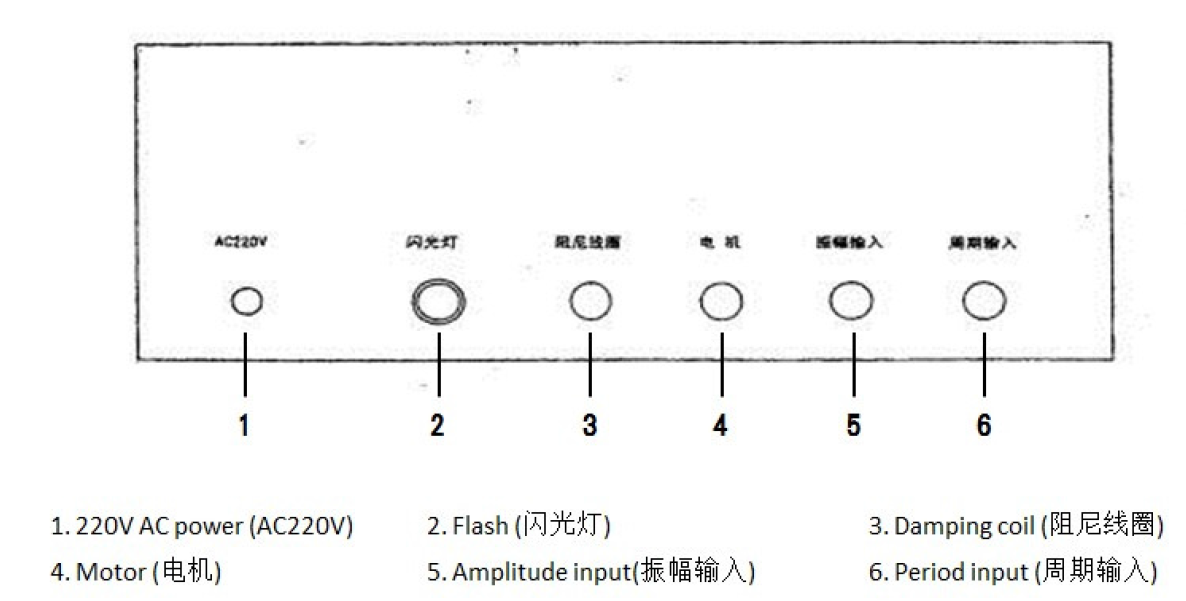
\includegraphics[scale=0.4]{P4.jpg}
\centering
\caption{The rear panel of the control box.}
\end{figure}
\item The value of $T$ should be the average period, and $ln\frac{\theta_i}{\theta_{i+5}}$should be obtained by the successive difference method as
$$\beta=\frac{1}{5T}ln\frac{\theta_i}{\theta_{i+5}}$$
\end{enumerate}
\subsection{$\theta_{st}$ vs. $\omega$ and $\varphi$ vs. $\omega$ Characteristics of Forced Oscillations}
\begin{enumerate}
\item Keep the \textbf{Damping Selection} at "2", and set the speed of the motor (record the
position of the motor knob in case you need to repeat the measurement). Record
the amplitude $\theta_{st}$, the period $T$, and the phase shift $\varphi$ when the oscillation reaches a steady state.
\item Repeat the steps above by changing the speed of the motor. It will result in a change
of the phase shift $\varphi$. To make your plots more accurate, you should collect more data when $\varphi$ and $\theta_{st}$ change rapidly. At least 15 data should be collected for plotting.
\item Choose \textbf{Damping Selection} "1" or "3". Repeat the above steps.
\item Plot the $\theta_{st}(\omega)$ characteristics, with $\omega/\omega_0$ on the horizontal axis and $\theta_{st}$ on the vertical axis. Two sets of data should be plotted on the same graph.
Plot the $\varphi(\omega)$ characteristics, with $\omega/\omega_0$ on the horizontal axis and $\varphi$ on the vertical axis. Two sets of data should be plotted on the same graph.
\end{enumerate}
\section{Calculation and Results}
\subsection{Measurement Data}
\subsubsection{Measurement of the Natural Frequency}
We first record the time of ten periods for four times.
\begin{table}[H]
\centering
\begin{tabular}{|c|c|}
\hline
        & 10T [s] $\pm$ 0.001 [s]       \\ \hline
1       & 15.733 \\ \hline
2       & 15.734 \\ \hline
3       & 15.733 \\ \hline
4       & 15.733 \\ \hline
Average & 15.733 \\ \hline
\end{tabular}
\caption{Measurement of the natural frequency}
\end{table}
\subsubsection{Measurement of the damping coefficient}
When we measure the damping coefficient, the damping selection is 2.
\begin{table}[H]
\centering
\begin{tabular}{|c|c|c|c|c|}
\hline
\multicolumn{2}{|c|}{Amplitude [$^o$] $\pm$ 1 [$^o$]} & \multicolumn{2}{c|}{Amplitude [$^o$] $\pm$ 1 [$^o$]} & ln($\theta_i/\theta_{i+5}$)  \\ \hline
$\theta_0$           &162           & $\theta_5$          &102           &0.4626  \\ \hline
$\theta_1$           &148           & $\theta_6$          &93           &0.4646  \\ \hline
$\theta_2$           &135        & $\theta_7$          &85           &0.4626  \\ \hline
$\theta_3$           &123        & $\theta_8$          &77           &0.4684  \\ \hline
$\theta_4$           &112           & $\theta_9$          &71           &0.4558  \\ \hline
\multicolumn{4}{|c|}{The average value of ln($\theta_i/\theta_{i+5}$)}                         &0.4628  \\ \hline
\end{tabular}
\caption{Measurement of the damping coefficient}
\end{table}
10$T$=15.814 [s] $\pm$ 0.001 [s]
\subsubsection{Damping Selection 2 Data for $\theta$ vs. $\omega$ and $\varphi$ vs. $\omega$ characteristics}
\begin{table}[H]
\centering
\begin{tabular}{|c|c|c|c|c|}
\hline
   & 10T [s] $\pm$ 0.001 [s] &$\omega/\omega_{0}$&$\varphi [^0] \pm 1 [^o]$&$\theta [^0] \pm 1 [^o]$     \\ \hline
1  & 15.162 &1.039& 164 & 41  \\ \hline
2  & 15.375 &1.024& 155 & 58  \\ \hline
3  & 15.519 &1.015& 145 & 81  \\ \hline
4  & 15.593 &1.010& 135 & 100 \\ \hline
5  & 15.644 &1.007& 126 & 118 \\ \hline
6  & 15.680 &1.004& 116 & 130 \\ \hline
7  & 15.710 &1.002& 106 & 139 \\ \hline
8  & 15.732 &1.001& 100 & 142 \\ \hline
9  & 15.748 &1.000& 95  & 144 \\ \hline
10 & 15.773 &0.998& 89  & 145 \\ \hline
11 & 15.792 &0.997& 84  & 144 \\ \hline
12 & 15.812 &0.996& 80  & 142 \\ \hline
13 & 15.860 &0.993& 71  & 136 \\ \hline
14 & 15.920 &0.989& 61  & 127 \\ \hline
15 & 15.981 &0.985& 54  & 116 \\ \hline
16 & 16.076 &0.980& 44  & 100 \\ \hline
17 & 16.232 &0.970& 32  & 77  \\ \hline
18 & 16.378 &0.962& 25  & 62  \\ \hline
19 & 16.582 &0.950& 18  & 48  \\ \hline
\end{tabular}
\caption{$\theta$ vs. $\omega$ and $\varphi$ vs. $\omega$ characteristics}
\end{table}
\subsubsection{Damping Selection 3 Data for $\theta$ vs. $\omega$ and $\varphi$ vs. $\omega$ characteristics}
\begin{table}[H]
\centering
\begin{tabular}{|c|c|c|c|c|}
\hline
   & 10T [s] $\pm$ 0.001 [s] &$\omega/\omega_{0}$&$\varphi [^0] \pm 1 [^o]$&$\theta [^0] \pm 1 [^o]$     \\ \hline
1  & 15.105 &1.043& 165 & 41  \\ \hline
2  & 15.367 &1.025& 156 &618  \\ \hline
3  & 15.532 &1.014& 145 & 87  \\ \hline
4  & 15.608 &1.009& 134 & 110 \\ \hline
5  & 15.655 &1.006& 121 & 132 \\ \hline
6  & 15.687 &1.004& 111 & 143 \\ \hline
7  & 15.706 &1.003& 105 & 148 \\ \hline
8  & 15.721 &1.002& 100 & 152 \\ \hline
9  & 15.734 &1.001& 95  & 154 \\ \hline
10 & 15.760 &0.999& 90 & 155 \\ \hline
11 & 15.778 &0.998& 85  & 154 \\ \hline
12 & 15.797 &0.997& 80  & 152 \\ \hline
13 & 15.825 &0.995& 74  & 148 \\ \hline
14 & 15.842 &0.994& 70  & 146 \\ \hline
15 & 15.893 &0.991& 62  & 136 \\ \hline
16 & 16.967 &0.986& 52  & 123 \\ \hline
17 & 16.071 &0.980& 43  & 103 \\ \hline
18 & 16.233 &0.970& 30  & 78 \\ \hline
19 & 16.439 &0.958& 21  & 59  \\ \hline
\end{tabular}
\caption{$\theta$ vs. $\omega$ and $\varphi$ vs. $\omega$ characteristics}
\end{table}
\subsection{Calculations}
\subsubsection{Natural Angular Frequency}
$$\omega_o=\frac{10\times2\pi}{T_{average}}=\frac{20\pi}{15.733}=3.99[rad/s]$$
\subsubsection{Damping Coefficient}
$$\beta=\frac{2}{T_{10}}ln\frac{\theta_i}{\theta_{i+5}}=\frac{2\times0.4628}{15.733}=0.059[s^{-1}]$$
\subsubsection{Graph for $\theta_{st}$ vs. $\omega$ Characteristics of Forced Oscillations}
\begin{figure}[H]
\centering
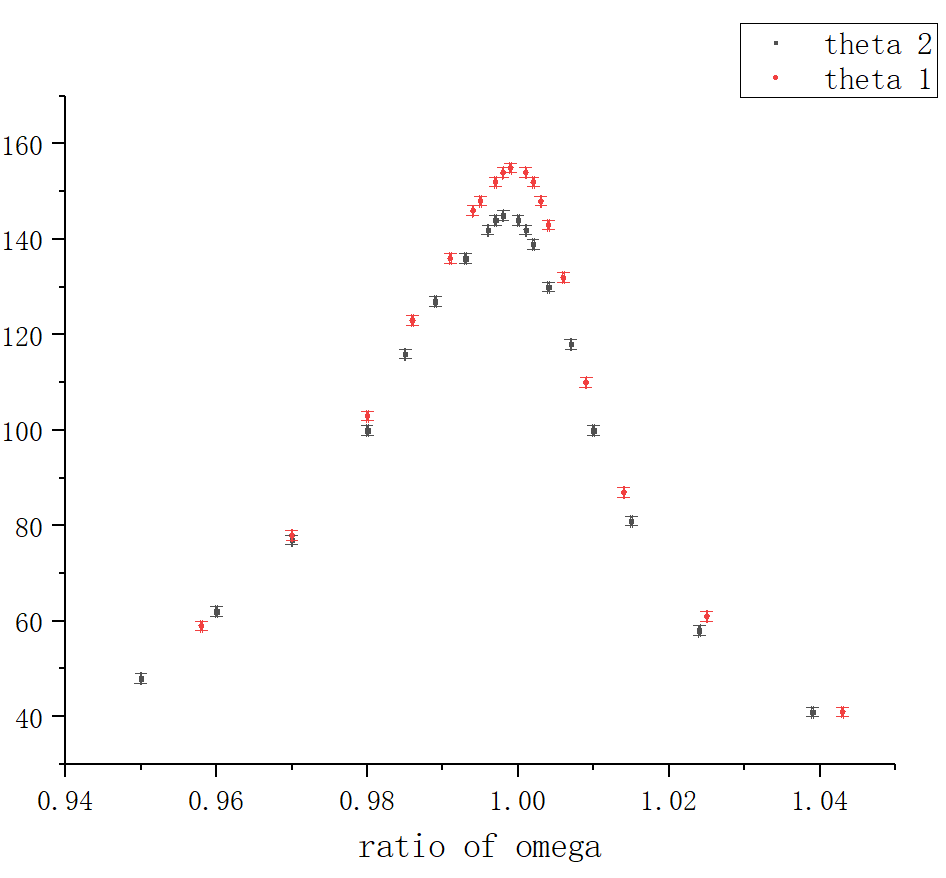
\includegraphics[scale=0.35]{P5.jpg}
\caption{ $\theta_{st}$ vs. $\omega$ Characteristics of Forced Oscillations}
\end{figure}
\subsubsection{Graph for $\varphi$ vs. $\omega$ Characteristics of Forced Oscillations}
\begin{figure}[H]
\centering
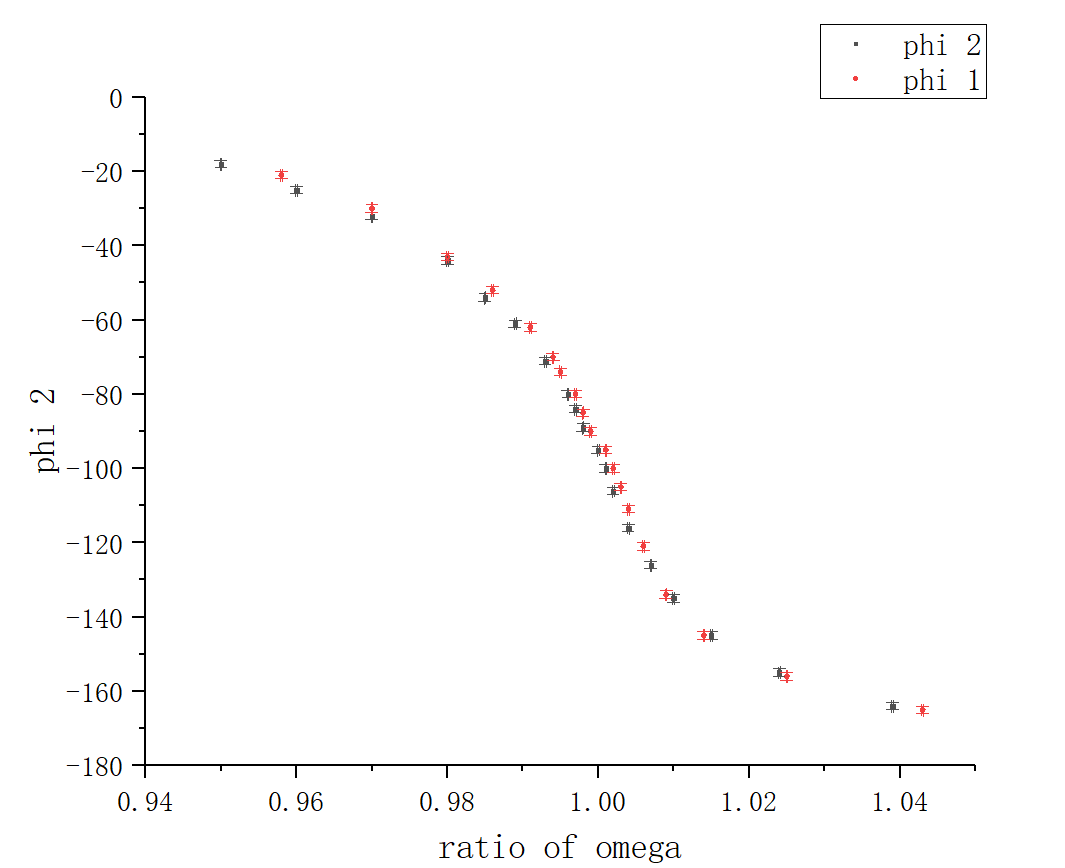
\includegraphics[scale=0.35]{P6.jpg}
\caption{ $\varphi$ vs. $\omega$ Characteristics of Forced Oscillations}
\end{figure}
\section{Measurement Uncertainty Analysis}
\subsection{Uncertainty of Natural Angular Frequency}
$$s_X=5\times10^{-4}$$
$$\bigtriangleup_A=\frac{S_Xt_{0.95}}{\sqrt{n}}=5\times10^{-4}\times1.59=7.95\times10^{-4}[s]$$
$$\bigtriangleup_B=0.001[s]$$
$$u_{10T}=\sqrt{\bigtriangleup_A^2+\bigtriangleup_B^2}=\sqrt{(7.95\times10^{-4}	)^2+(0.001)^2}=1.28\times10^{-3}[s]$$
$$\omega_0=\frac{20\pi}{T_{10}}$$
$$u_{\omega}=\frac{\partial{\omega_0}}{\partial{T_{10}}}\cdot u_T=\frac{20\pi}{15.733^2}\times1.28\times10^{-3}=3.25\times10^{-4}[rad/s]$$
$$u_r=\frac{u_{\omega}}{\omega_0}\times100\%=\frac{3.25\times10^{-4}}{4.00}\times100\%=0.01\%$$
\subsection{Uncertainty of Damping Coefficient}
\subsubsection{Uncertainty of ln($\theta_i/\theta_{i+5}$)}
$$\textsf{ln}(\theta_i/\theta_{i+5})=0.4628$$
$$s_X=4.57\times10^{-3}$$
$$\bigtriangleup_A=4.57\times10^{-3}\times1.204=5.51\times10^{-3}$$
$$\bigtriangleup_{B_i}=\sqrt{(\frac{\partial{ln(\theta_i/\theta_{i+5})}}{\partial{\theta_i}}\cdot u_{theta_i})^2+(\frac{\partial{ln(\theta_i/\theta_{i+5})}}{\partial{\theta_{i+5}}}\cdot u_{theta_{i+5}})^2}=\sqrt{(\frac{u_{\theta_i}}{\theta_i})^2+(\frac{u_{\theta_{i+5}}}{\theta_{i+5}})^2}$$
When i=0:
$$\bigtriangleup_{B_0}=\sqrt{(\frac{1}{162})^2+(1/102)^2}=0.012$$
\begin{table}[H]
\centering
\begin{tabular}{|c|c|}
\hline
i  &$\bigtriangleup_B$  \\ \hline
0  &0.012  \\ \hline
1  &0.013  \\ \hline
2  &0.014  \\ \hline
3  &0.015  \\ \hline
4  &0.017  \\ \hline
average &0.014\\ \hline
\end{tabular}
\caption{$\bigtriangleup_{B_i}$}
\end{table}
$$u=\sqrt{\bigtriangleup_A^2+\bigtriangleup_B^2}=\sqrt{(5.51\times10^{-3})^2+0.014^2}=0.015$$
\subsubsection{Uncertainty of Damping Coefficient}
$$\beta=\frac{2}{T_{10}}ln\frac{\theta_i}{\theta_{i+5}}$$
$$u_{\beta}=2\sqrt{(\frac{0.4628}{15.814^2}\times0.001)^2+(\frac{0.015}{15.814})^2}=1.9\times10^{-3}[s^{-1}]$$
$$u_r=\frac{u_{\beta}}{\beta}\times100\%=\frac{1.9\times10^{-3}}{0.059}\times100\%=3.22\%$$
\subsection{Uncertainty of $\omega/\omega_0$}
$$u_1=\sqrt{(\frac{u_{\omega}}{\omega_0})^2+(\frac{u_{\omega_0}\cdot\omega}{\omega_0}^2)^2}=\sqrt{(\frac{3\times10^{-4}}{4})^2+(\frac{3\times10^{-4}\times4.144}{4}^2)^2}=1.1\times10^{-4}$$
$$u_r=\frac{1.1\times10^{-4}}{1.039}\times100\%=0.01\%$$
\subsection{Uncertainty of Data for $\theta_{st}$ vs. $\omega$ in Section 2}
The uncertainty can be calculated similarly like natural angular frequency.
\begin{table}[H]
\centering
\begin{tabular}{|c|c|c|c|c|c|c|}
\hline
   &$\omega[rad/s]$ &$u_{\omega}[rad/s]$&$u_r$&$\omega/\omega_0$&u&$u_r$ \\ \hline
1  & 4.144 & $3\times10^{-4}$ & $0.01\%$&1.039&$1.1\times10^{-4}$&0.01$\%$ \\ \hline
2  & 4.087 & $3\times10^{-4}$ & $0.01\%$&1.024&$1.1\times10^{-4}$&0.01$\%$ \\ \hline
3  & 4.049 & $3\times10^{-4}$ & $0.01\%$&1.015&$1\times10^{-4}$&0.01$\%$\\ \hline
4  & 4.029 & $3\times10^{-4}$ & $0.01\%$&1.010&$1\times10^{-4}$&0.01$\%$ \\ \hline
5  & 4.016 & $3\times10^{-4}$ & $0.01\%$&1.007&$1\times10^{-4}$&0.01$\%$ \\ \hline
6  & 4.007 & $3\times10^{-4}$ & $0.01\%$&1.004&$1\times10^{-4}$&0.01$\%$ \\ \hline
7  & 3.999 & $3\times10^{-4}$ & $0.01\%$&1.002&$1\times10^{-4}$&0.01$\%$ \\ \hline
8  & 3.994 & $3\times10^{-4}$ & $0.01\%$&1.001&$1\times10^{-4}$&0.01$\%$ \\ \hline
9  & 3.990 & $3\times10^{-4}$  & $0.01\%$&1.000&$1\times10^{-4}$&0.01$\%$ \\ \hline
10 & 3.984 & $3\times10^{-4}$  & $0.01\%$&0.998&$1\times10^{-4}$&0.01$\%$ \\ \hline
11 & 3.792 & $3\times10^{-4}$  & $0.01\%$&0.997&$1\times10^{-4}$&0.01$\%$ \\ \hline
12 & 3.974 & $3\times10^{-4}$  & $0.01\%$&0.996&$1\times10^{-4}$&0.01$\%$ \\ \hline
13 & 3.962 & $3\times10^{-4}$  & $0.01\%$&0.993&$1\times10^{-4}$&0.01$\%$ \\ \hline
14 & 3.947 & $2\times10^{-4}$  & $0.01\%$&0.989&$1\times10^{-4}$&0.01$\%$ \\ \hline
15 & 3.931 & $2\times10^{-4}$  & $0.01\%$&0.985&$1\times10^{-4}$&0.01$\%$ \\ \hline
16 & 3.908 & $2\times10^{-4}$  & $0.01\%$&0.980&$1\times10^{-4}$&0.01$\%$ \\ \hline
17 & 3.871 & $2\times10^{-4}$  & $0.01\%$&0.970&$1\times10^{-4}$&0.01$\%$  \\ \hline
18 & 3.836 & $2\times10^{-4}$  & $0.01\%$&0.962&$1\times10^{-4}$&0.01$\%$  \\ \hline
19 & 3.789 & $2\times10^{-4}$  & $0.01\%$&0.950&$1\times10^{-4}$&0.01$\%$  \\ \hline
\end{tabular}
\caption{$\theta$ vs. $\omega$ and $\varphi$ vs. $\omega$ characteristics}
\end{table}
\subsection{Uncertainty of Data for $\theta_{st}$ vs. $\omega$ in Section 1}
The uncertainty can be calculated similarly like natural angular frequency.
\begin{table}[H]
\centering
\begin{tabular}{|c|c|c|c|c|c|c|}
\hline
   &$\omega[rad/s]$ &$u_{\omega}[rad/s]$&$u_r$&$\omega/\omega_0$&u&$u_r$ \\ \hline
1  & 4.160 & $3\times10^{-4}$ & $0.01\%$&1.043&$1.1\times10^{-4}$&0.01$\%$ \\ \hline
2  & 4.089 & $3\times10^{-4}$ & $0.01\%$&1.025&$1.1\times10^{-4}$&0.01$\%$ \\ \hline
3  & 4.045 & $3\times10^{-4}$ & $0.01\%$&1.014&$1\times10^{-4}$&0.01$\%$\\ \hline
4  & 4.026 & $3\times10^{-4}$ & $0.01\%$&1.009&$1\times10^{-4}$&0.01$\%$ \\ \hline
5  & 4.014 & $3\times10^{-4}$ & $0.01\%$&1.006&$1\times10^{-4}$&0.01$\%$ \\ \hline
6  & 4.005 & $3\times10^{-4}$ & $0.01\%$&1.004&$1\times10^{-4}$&0.01$\%$ \\ \hline
7  & 4.000 & $3\times10^{-4}$ & $0.01\%$&1.003&$1\times10^{-4}$&0.01$\%$ \\ \hline
8  & 3.997 & $3\times10^{-4}$ & $0.01\%$&1.002&$1\times10^{-4}$&0.01$\%$ \\ \hline
9  & 3.993 & $3\times10^{-4}$  & $0.01\%$&1.001&$1\times10^{-4}$&0.01$\%$ \\ \hline
10 & 3.987 & $3\times10^{-4}$  & $0.01\%$&0.999&$1\times10^{-4}$&0.01$\%$ \\ \hline
11 & 3.982 & $3\times10^{-4}$  & $0.01\%$&0.998&$1\times10^{-4}$&0.01$\%$ \\ \hline
12 & 3.977 & $3\times10^{-4}$  & $0.01\%$&0.997&$1\times10^{-4}$&0.01$\%$ \\ \hline
13 & 3.970 & $3\times10^{-4}$  & $0.01\%$&0.995&$1\times10^{-4}$&0.01$\%$ \\ \hline
14 & 3.966 & $3\times10^{-4}$  & $0.01\%$&0.994&$1\times10^{-4}$&0.01$\%$ \\ \hline
15 & 3.953 & $2\times10^{-4}$  & $0.01\%$&0.991&$1\times10^{-4}$&0.01$\%$ \\ \hline
16 & 3.935 & $2\times10^{-4}$  & $0.01\%$&0.986&$1\times10^{-4}$&0.01$\%$ \\ \hline
17 & 3.910 & $2\times10^{-4}$  & $0.01\%$&0.980&$1\times10^{-4}$&0.01$\%$  \\ \hline
18 & 3.871 & $2\times10^{-4}$  & $0.01\%$&0.970&$1\times10^{-4}$&0.01$\%$  \\ \hline
19 & 3.822 & $2\times10^{-4}$  & $0.01\%$&0.958&$1\times10^{-4}$&0.01$\%$  \\ \hline
\end{tabular}
\caption{$\theta$ vs. $\omega$ and $\varphi$ vs. $\omega$ characteristics}
\end{table}
\section{Conclusion and Discussion}
\subsection{Conclusion}
In this exercise, I have a rough idea about the damped and driven oscillations. I also learn the usage of resonator.	Also, I calculate the natural angular frequency and damping coefficient. $\omega_0=4.00\pm3.25\times10^{-4}[s^{-1}]$ with relative error $0.01\%$.
$\beta=0.059\pm1.9\times10^{-3}[s^{-1}]$ with relative error $3.22\%$
\par I also measured the data of $10T$, $\varphi$, and $\theta$ to draw graphs for $\theta$ vs. $\omega$ and $\varphi$ vs. $\omega$ characteristics. The figure is similar to the first picture in figure 1. $\theta$ reaches its maximum value when $\omega/\omega_0\approx1$, and $\beta_1$ is large than $\beta_2$.
\subsection{Discussion}
\subsubsection{Suggestions and Improvement}
At first, we did the exercise quite slow because it's hard for us to find the relation between driven force and $\varphi$. I think I should be more familiar with the resonator in advance.
\par Since the most important part of the graph is when $\omega$ is close to $\omega_0$, which means $\varphi$ is close to 90, so we measured more data at that time. 
\subsubsection{Error Analysis}
$\beta$'s relative error is $3.22\%$, which is quite large and can't be neglected. I think it's air damping that lead to such large error.
\par The $\omega_0$'s error is not so large, I think it comes from the resonator itself.
\section{Data Sheet}
Data sheet is attach to the report
\section{Reference}
\begin{enumerate}[-]
\item Young, H.D., Freedman R.A. University Physics. Chapter 21,23,24.
\item Qin Tian, Zeng Ming, Zhao Xijian, Krzyzosiak,M. Lab Manual of Exercise 5.
\item Qin Tian, Zeng Ming, Zhao Xijian, Krzyzosiak,M. Handbook-Uncertainty Analysis.
\end{enumerate}
\end{document}